\begin{enumerate}
\def\labelenumi{\arabic{enumi}.}
\tightlist
\item
  Abstract
\item
  Introduction

  \begin{itemize}
  \tightlist
  \item
    Motivation
  \item
    Current State
  \item
    Prior Work
  \item
    Expectation
  \end{itemize}
\item
  Object Caches

  \begin{itemize}
  \tightlist
  \item
    Purpose
  \item
    Desired qualities
  \item
    Design \& Implementations
  \item
    Performance measurements and methodology
  \item
    Current State of caches \& Usage in industry
  \end{itemize}
\item
  Testing Methodology

  \begin{itemize}
  \tightlist
  \item
    Define Quality of Service (99th \textless{} 1ms?)
  \item
    What are we interested in (in terms of stats)
  \item
    Testing setup
  \item
    Comparison to testbeds in other papers
  \item
    Memtier \& comparison to others
  \item
    Memtier

    \begin{itemize}
    \tightlist
    \item
      Justify why memtier
    \item
      Outline how memtier works
    \end{itemize}
  \item
    Open loop vs closed loop
  \item
    Discuss error conditions and repeatability
  \end{itemize}
\item
  Memcached

  \begin{itemize}
  \tightlist
  \item
    Outline

    \begin{itemize}
    \tightlist
    \item
      What memcached is
    \item
      Who/where it is used
    \item
      How would a typical memcached setup look like
    \item
      Link with paper on FB memcached setup and workloads
    \end{itemize}
  \item
    Design decisions

    \begin{itemize}
    \tightlist
    \item
      Multi-threaded
    \item
      Locks
    \item
      Memory allocation
    \end{itemize}
  \item
    Important configuration options and defaults
  \item
    Memcached Throughput under QoS

    \begin{itemize}
    \tightlist
    \item
      Latency vs Throughput
    \item
      CPU vs QoS
    \end{itemize}
  \item
    Memcached thread scalability

    \begin{itemize}
    \item ~
      \section{of threads vs QoS}\label{of-threads-vs-qos}
    \item
      Thread pinning
    \item
      Rx/Tx queues
    \end{itemize}
  \item
    Memcached process scalability

    \begin{itemize}
    \item ~
      \section{of processes vs QoS}\label{of-processes-vs-qos}
    \end{itemize}
  \item
    Memcached and Group Size

    \begin{itemize}
    \tightlist
    \item
      based on
      \href{http://ieeexplore.ieee.org/stamp/stamp.jsp?tp=\&arnumber=7095781}{Where
      does the time go?}
    \end{itemize}
  \item
    Summary

    \begin{itemize}
    \tightlist
    \item
      Maximum throughput under QoS with threads/processes/Rx/Tx configs
    \item
      Cross-link with literature and justify numbers
    \item
      Summarize performance
    \end{itemize}
  \end{itemize}
\item
  Redis

  \begin{itemize}
  \tightlist
  \item
    Outline

    \begin{itemize}
    \tightlist
    \item
      What it is
    \item
      What does it do - feature set
    \item
      Who would/does use it
    \item
      Why would someone choose it over other object caches
    \item
      How does a typical redis deployment look like
    \end{itemize}
  \item
    Redis design

    \begin{itemize}
    \tightlist
    \item
      Philosophy

      \begin{itemize}
      \tightlist
      \item
        Simple is better
      \item
        Easier to reason about
      \end{itemize}
    \item
      Single threaded/lock-free
    \item
      Persistence
    \item
      No default sharding
    \end{itemize}
  \item
    Setup and configuration options
  \item
    Benchmarks and results

    \begin{itemize}
    \tightlist
    \item
      TODO: Similar benchmarks as with memcached
    \end{itemize}
  \end{itemize}
\item
  Evaluation

  \begin{itemize}
  \tightlist
  \item
    M vs R in terms of latency under QoS
  \item
    M vs R in terms of throughput under QoS
  \item
    M vs R in terms of total throughput outside QoS (?)
  \end{itemize}
\end{enumerate}

Abstract goes here.. \# Motivation

The world is increasingly demanding better and faster access to
information. With advances in commodity hardware, and the rise of
commodity computing, it has provided means to address one of the ways to
increase performance. The proposed ways are as follows - a) Word harder,
b) Work smarter and c) Get help, as outlined in {[}G. Pfsiter, In Search
of Clusters{]}. Commodity computing has been able to address how to get
help, namely distribution of work across machines. Caches attempt to
address how to work smarter, particularly how to perform less
computation.

The increase of distributed computing has also introduced new challenges
such as consistency and resiliency of the network under question. The
same challenges are having to be addressed across the application stack,
including the caching mechanism. With advances in hardware performance
and also the size of networks, it will increasingly essential to be able
to make caching systems as effective as possible. Inherently,
multi-threded and distributed computing poses

With the increased usage of commodity computing {[}G. Pfister, In Search
of Clusters, Prentice Hall PTR, 1998{]}, it has become possible to
utilize larger

\begin{enumerate}
\def\labelenumi{\arabic{enumi}.}
\tightlist
\item
  We need to be able to scale on a single server better
\item
  We need to be able to scale across servers better
\item
  We need to see if multi-threaded approach is better than single
  threaded with simpler system \# Memory Object Caches
\end{enumerate}

\subsection{Purpose}\label{purpose}

In the traditional sense of way, a cache is a data structure which
stores the results of a computation for later retrieval. Generally, a
result of a computation is stored against a \emph{key} with a
\emph{value} representing the computed result. When retrieving data from
the cache, we say there is a \emph{hit} if the key can be found in the
cache and a \emph{miss} otherwise. Caching is widely used across the
hardware and software stack. For example, modern processors utilize a
CPU cache to increase the speed of memory lookup. Similarly, a cache can
also be found inside a web server to speed up retrieval of results from
the server.

An object cache is a general purpose cache, generally designed as a
standalone application, which provides an interface to cache any type of
object - for example, an object cache can store large text documents,
small tweets or binary data such as images.

A memory object cache is an object with additioanal restriction where
data is only stored in the available (or assigned) RAM of the computer.
This restriction is important as storing data on hardware slower than
RAM would incure too high of a latency and would degrade quality of
service.

Both Memcached and Redis are open-source implementations of memory
object caches.

\subsection{Desired qualities}\label{desired-qualities}

TODO

\subsection{Design \& Implementations}\label{design-implementations}

TODO

\subsection{Performance measurements and
methodology}\label{performance-measurements-and-methodology}

TODO

\subsection{Current State of caches \& Usage in
industry}\label{current-state-of-caches-usage-in-industry}

TODO

\section{Methodology}\label{methodology}

\begin{itemize}
\tightlist
\item
  Quality of Service (99th \textless{} 1ms?)
\item
  Testing setup
\item
  Comparison to testbeds in other papers
\item
  Memtier \& comparison to others
\item
  Justify Memtier
\item
  Open loop vs closed loop
\item
  What are we interested in
\item
  Discuss error conditions and repeatability
\end{itemize}

\subsection{Quality of Service}\label{quality-of-service}

Firstly, it is important to define an acceptale quality of service (QoS)
for an object cache in question. Distributed systems are increasingly
more popular with responses to requests being a composition of smaller
responses from respective sub-systems. Given all sub-systems must return
a response before the complete response is serviced to the requestor,
the slowest of all smaller responses will determine the overall response
time. Frequently, the QoS aimed for is sub-1ms latency. Similar target
is used by Leverich and Kozyrakis {[}1{]}. Therefore, in this study the
aim will be to achieve tail latency under 1ms, that is in 99\% of cases.

\subsection{Testing setup}\label{testing-setup}

The performance benchmarks are run on 8 machines with the following
configuration: 6 core Intel(R) Xeon(R) CPU E5-2603 v3 @ 1.60GHz {[}2{]},
8 GB RAM and 1Gb/s Network Interface Controller (NIC).

All the hosts are connected to a Pica8 P-3297 {[}3{]} switch with 48
1Gbps ports with a star as the network topology. A single host is used
to run an object cache system while the remaining seven are used to
generate workloads against the server.

\subsection{Workload generation}\label{workload-generation}

Workload for the cache server is generated using Memtier Benchmark
{[}4{]}. The Memtier Benchmark provides a configurable parallel workload
generation for both Memcached and Redis. Additionally, it allows for a
high level of configrability.

\subsubsection{Memtier Benchmark
Behavior}\label{memtier-benchmark-behavior}

Memtier Benchmark provides various paramters allowing for a variable
configuration. As part of the configration, the user is allowed to
specify the number of threads and the number of connections per each
thread memtier should make. The standard lifecycle of each thread is as
follows:

\begin{enumerate}
\def\labelenumi{\arabic{enumi}.}
\tightlist
\item
  Set up n connection configurations
\item
  For each connection configuration, initiate the connection over the
  desired protocol (default: TCP)
\item
  Make a request
\item
  Tear down the connection
\item
  Repeat iterations
\end{enumerate}

\subsubsection{Open loop vs Closed loop}\label{open-loop-vs-closed-loop}

Memtier is closed loop

\begin{itemize}
\tightlist
\item
  {[}1{]} Reconciling High Server Utilization and Sub-millisecond
  Quality-of-Service
\item
  {[}2{]} {[}Intel(R) Xeon(R)
  E5-2603{]}(http://ark.intel.com/products/64592/Intel-Xeon-Processor-E5-2603-10M-Cache-1\_80-GHz-6\_40-GTs-Intel-QPI)
\item
  {[}3{]} {[}Pica8
  Datasheet{]}(http://www.pica8.com/wp-content/uploads/2015/09/pica8-datasheet-48x1gbe-p3297.pdf)
\item
  {[}4{]} {[}Memtier
  Benchmark{]}(https://github.com/RedisLabs/memtier\_benchmark)
\end{itemize}

\section{Memcached}\label{memcached}

\subsection{Outline}\label{outline}

Memcached is a simple distributed memory object cache {[}1{]}. It
provides a simple interface to allow systems to store, retrieve and
update the contents of the cache. It is developed as an open source
project and has been extensively studied in the literature. Often, it is
used as an application of choice to benchmark system configurations in
terms of network throughput, memory allocation policies and more
generally to understand how a system performs under stress. Furthermore,
it is often used as an application for experiementation and
implementation of next generation technology such as the use of a Field
Programmable Gate Array (FPGA) {[}2{]}.

The API supported by memcached is straightforward. Memcached philosophy
is to execute commands against an item of the cache rather than
manipulate the cache as a whole. Out of the box, memcached supports the
following operations for retrieval: \emph{set, add, replace, append,
prepend and cas} {[}3{]}. Similarly, memcached supports the following
storage commands: \emph{get, gets, delete and incr/decr} {[}3{]}. The
API is deliberetly designed to be intuitive making the effect of an
action predictable. The action labelled \emph{cas} perhaps requires
further clarification, however. The full action name is \emph{check and
set}, data is stored only if the comparison with current value fails.

Memcached has grown to be a very popular general purpose cache in the
industry. Currently, Facebook is considered to have the largest
deployment of memcached in production {[}4{]} while there are many other
companies utilizing large deployments of memcached as building blocks of
their infrastructure, these include Twitter{[}5{]}, Amazon {[}6{]} and
many others.

In the simplest memcached deployment, an instance of memcached can be
run alongside another application, for example a web server. In such a
setup, no network communication is required and the web server can talk
to memcached over a local unix socket. This configuration has
disadvantages, for example, horizontally scaling the web server would
require another instance of the cache to be deployed as well potentially
leading decreased cache hit rate.

More complicated deployments generally utilize a memcached instance
running on a seperate host with all instances of, for example, web
servers communicating with a single memcached host. The advantage of
such a setup is decreased coupling and increased potential for
scalability by adding more instances of both web server and memcached.

In the largest scenarios, such as Facebook, a large number of client
applications are talking to a number of memcached clusters responsible
for a given type of information. Effectively creating a data layer where
any client application can request information from any pool increasing
modularity and interoperability of the infrastructure. {[}Ref?{]}

(Diagram to illustrate deployments here?)

To illustrate the importance and also the size of a memcached
deployment, a workload charasterization from Facebook will be used
{[}7{]}. Figure below illustrates the throughput observed in a Facebook
pools deployed over the course of 7 days. We can observe that the total
number of requests is close to 1.26 trillion requests over 7 days, this
is on average 2.08 million requests a second. The volume itself is
large, however, considering Facebook has 1.44 billion active monthly
users {[}8{]}, however, it does demonstrate the scale at which Facebook
utilizes memcached and the impact memcached has on ability to scale and
handle traffic at Facebook.

\begin{figure}[htbp]
\centering
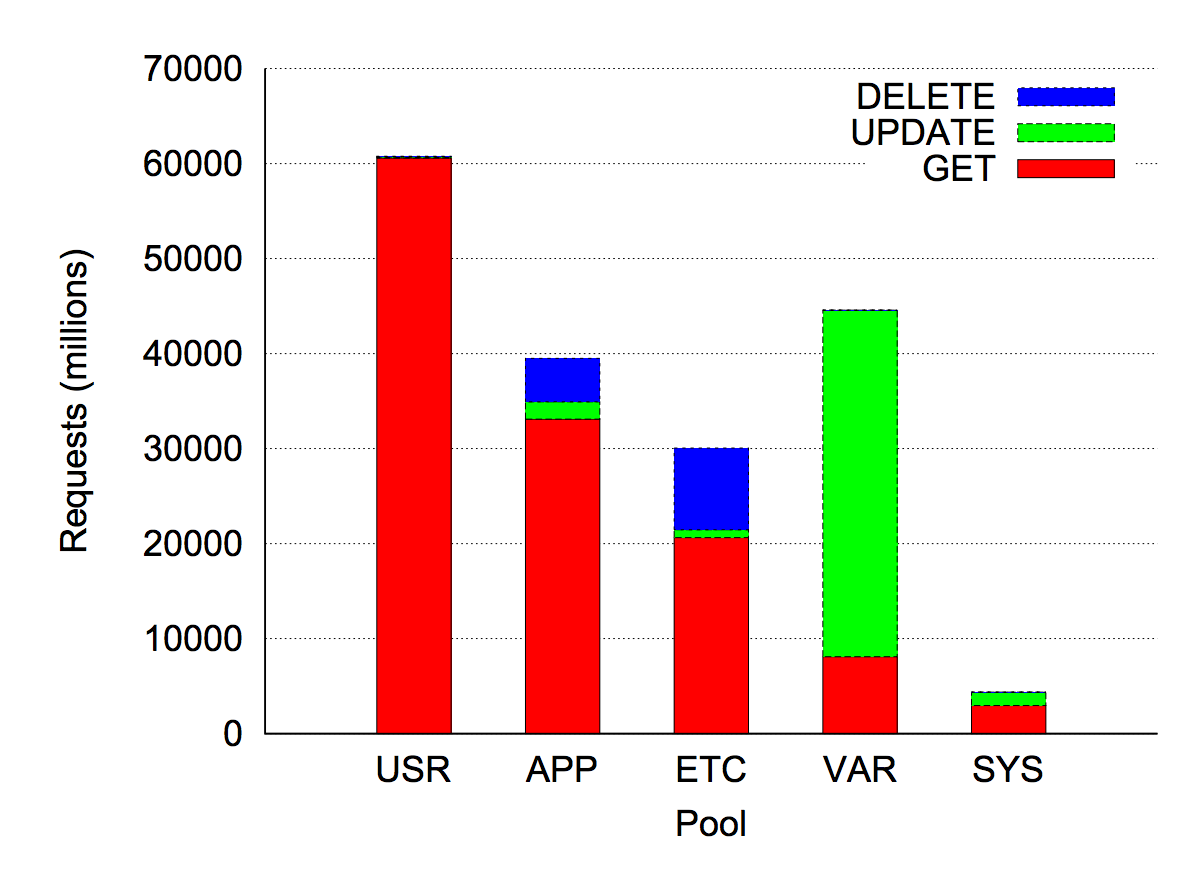
\includegraphics{./res/5_facebook_pool_ops.png}
\caption{Facebook Pools Operations}
\end{figure}

\subsection{Design decisions}\label{design-decisions}

From the early development stages, memcached has been designed in a
client-server architecture. Therefore, a memcached applications receives
a command based on its API, executes the command and returns a reply to
the client. Memcached is deliberetly designed as a standalone
application rather than being integrated into a particular
system/framework in order to be able to act as a general purpose cache
and allow decoupling of responsibilities in an system architecture.

Memcached implements its distributed protocol through consistent hashing
on the client side. Therefore, keeping logic on the server side minimal
and allowing the clients to figure out which instance to talk to. In
order to further improve horizontal scaling properties of memcached,
solutions such as Twemproxy {[}9{]} exist to support scalability of an
individual shard of a distributed memcached deployment.

The memory requirements of memcached are specified as a configration
option before the memcached application is started. Knowing an upper
bound on the amount of memory memcached can use allows memcached to
claim the required memory and handle memory management itself rather
than using \emph{malloc, free or realloc}. \emph{Slabs} are structured
to be blocks of memory with 1MB allocated to them. Each slab belogns to
a \emph{slab group} which determines the size of each chunk inside the
slab. By default, the minimum chunk size is 80 bytes with a hard maximum
of 1MB. The growth factor between different slab groups is 1.25. Within
each slab group, a Least Recently Used (LRU) eviction policy is employed
effectively evicting entries least recently used within a similar memory
requirement first.

Private networks are the intended target of memcached where applications
designed to be publicly exposed access memcached on behalf of the
requestor rather than exposing the cache directly. By default, memcached
provides access to all entries of the cache for all clients but there is
also an option to be used with a Simple Authentication and Security
Layer (SASL) option.

Memcached is a multi-threaded application which introduces the
requirement to lock resources during critical sections in order to
prevent race conditions. The main reason for designing multi-threaded
applications is improve performance. Parsing a request and understanding
the nature of a request can be in parallel with data retrieval from
memory while a response is being constructed, all in their own
respective threads. However, in order to achieve the apprearance of
operation atomicity, a mutual exclusion lock is required. A request
lifecycle is as follows {[}10{]}:

\begin{enumerate}
\def\labelenumi{\arabic{enumi}.}
\tightlist
\item
  Requests are received by the Network Interface Controller (NIC) and
  queued
\item
  \emph{Libevent} receives the request and delivers it to the memcached
  application
\item
  A worker thread receives a request, parses it and determines the
  command required
\item
  The \emph{key} in the request is used to calculate a hash value to
  access the memory location in \emph{O(1)}
\item
  Cache lock is acquired \emph{(entering critical section)}
\item
  Command is processed and LRU policy is enforced
\item
  Cache lock is released \emph{(leaving critical section)}
\item
  Response is constructed and transmitted
\end{enumerate}

Given the outline above, we can see that steps 5. to 7. transform the
parallel nature of processing a request into a serial process.
Optimizations to the critical section have been well studied but it
should be noted that memcahed suffers from overheads related to global
lock acquizition and release.

\subsection{Configuration options}\label{configuration-options}

Memcached provides a convenient command line configration options to
tweak the performance of memcached through various parameters, the most
important ones are: * \emph{-d} runs application in daemon mode *
\emph{-p } binds application to a port (18080 by default) * \emph{-m }
defines how much memory to allocate to memcached.

Given the host hardware has 8GB memory, 6GB will be allocated to
memcached to leave some memory for the underlying operating system.
Throughout this paper, mostly options outlined above will be utilized.
Where applicable, further settings will be explained.

\subsection{Throughput under QoS}\label{throughput-under-qos}

Firstly, to establish a baseline it is essential to understand memcached
behavior under high utilization. In order to establish this baseline, a
default configuration of memcached will be used with a variable workload
generated by the clients. Therefore, the memcached server is started
with the following configuration
\texttt{memcached\ -d\ -p\ 11120\ -m\ 6144} setting the port and
allocating 6GB of memory to memcached. Each memtier instance is
configured with variable number of connections and treads such that the
total number of connections (threads * number of connections per thread)
is progressively increased. Memtier instances use the following
configuration:
\texttt{memtier\ -s\ nsl200\ -p\ 11120\ -\/-test-time=60\ -c\ \textless{}number\ of\ clients\textgreater{}\ -t\ \textless{}number\ of\ threads\textgreater{}\ -P\ memcache\_binary\ -\/-random-data\ -\/-key-minimum=100\ -\/-key-maximum=10000}.
The key size is capped between 100 and 10000 in order to simulate a
realistic hit rate.

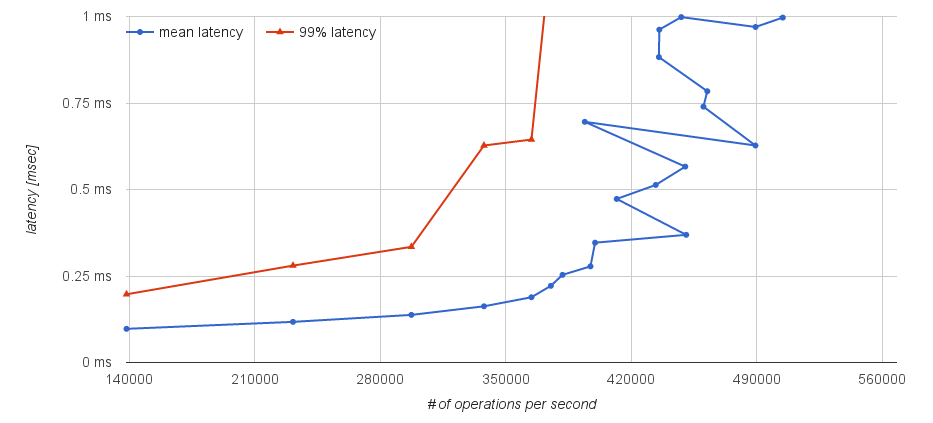
\includegraphics{./res/5_baseline_latency_vs_ops.png} \emph{Throughput
vs mean and 99th perecentile latency}

From the figure above, we can see that both the mean latency and the
99th perecentile latency increases linearly until we reach a saturation
point at which point each increase in throughput is met with a much
larger increase in latency. Additionally, we can see that the highest
throughput achieved with 99th percentile under 1ms is 375k operations
per second. This corresponds to 84 simultaneous connections, or 12
connections per each client. This is similar to benchmarks used in the
literature {[}11{]}.

\begin{figure}[htbp]
\centering
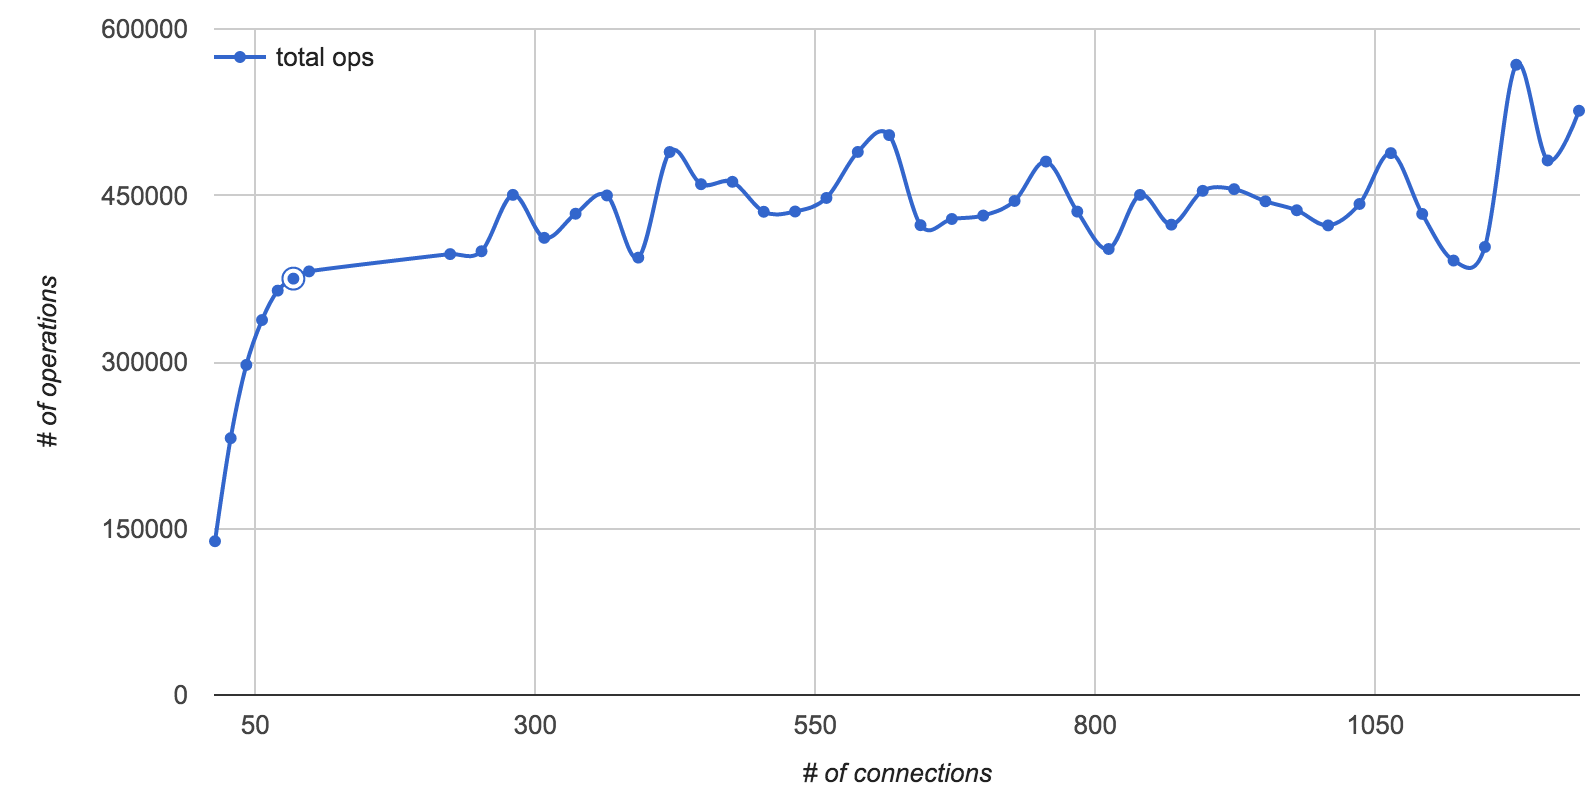
\includegraphics{./res/5_baseline_connections_vs_ops.png}
\caption{Memcached Default Configuration Baseline Connections vs Ops}
\end{figure}

In order to further understand the impact of an increase in the number
of connections, consider the figure above comparing the number of
connections with the number of operations executed. We can see that
memcached scales well until we reach a saturation point at around 84
connections (highlighted). A further increase in the number of
connections is met with a much lower increase in the total number of
operations performed. The shaded segments under the curve represent the
portion of CPU time spent processing memcached (blue) and in the system
(red). Furthermore, we can see that when we reach the saturation point,
memcached CPU usage remains consistent while all the remaining time is
spent in the system. The system requires a large number of resources to
process the incoming network requests and to process the outgoing
requests from memcached. Finally, the diagram also demonstrates that
memcached performance is tightly linked with the performance of the
network stack and the underlying hardware responsible for handling
incoming and outgoing communication. This is consistent with findings in
other papers {[}12{]}.

\subsection{Memcached Thread
Scalability}\label{memcached-thread-scalability}

Memcached is designed to process requests in parallel and therefore a
reasonable first step in scaling memcached is to provision more threads
for the application. Considering that the benchmarking setup has a
six-core processor, it is reasonable to expect the best performance when
running memcached with six threads.

Utilizing findings from the previous section, configuration with 84
connections can be used to generate consistent load while the number of
threads provisioned for memcached is increased. Therefore, each client
is setup as follows:
\texttt{memtier\ -s\ nsl200\ -p\ 11120\ -\/-test-time=30\ -c\ 6\ -t\ 2\ -P\ memcache\_binary\ -\/-random-data\ -\/-key-minimum=100\ -\/-key-maximum=10000}
and the server is configured with
\texttt{memcached\ -d\ -p\ 11120\ -m\ 6144\ -t\ \textless{}threads\textgreater{}}
where \texttt{\textless{}threads\textgreater{}} varies between 1 and 35.

\begin{figure}[htbp]
\centering
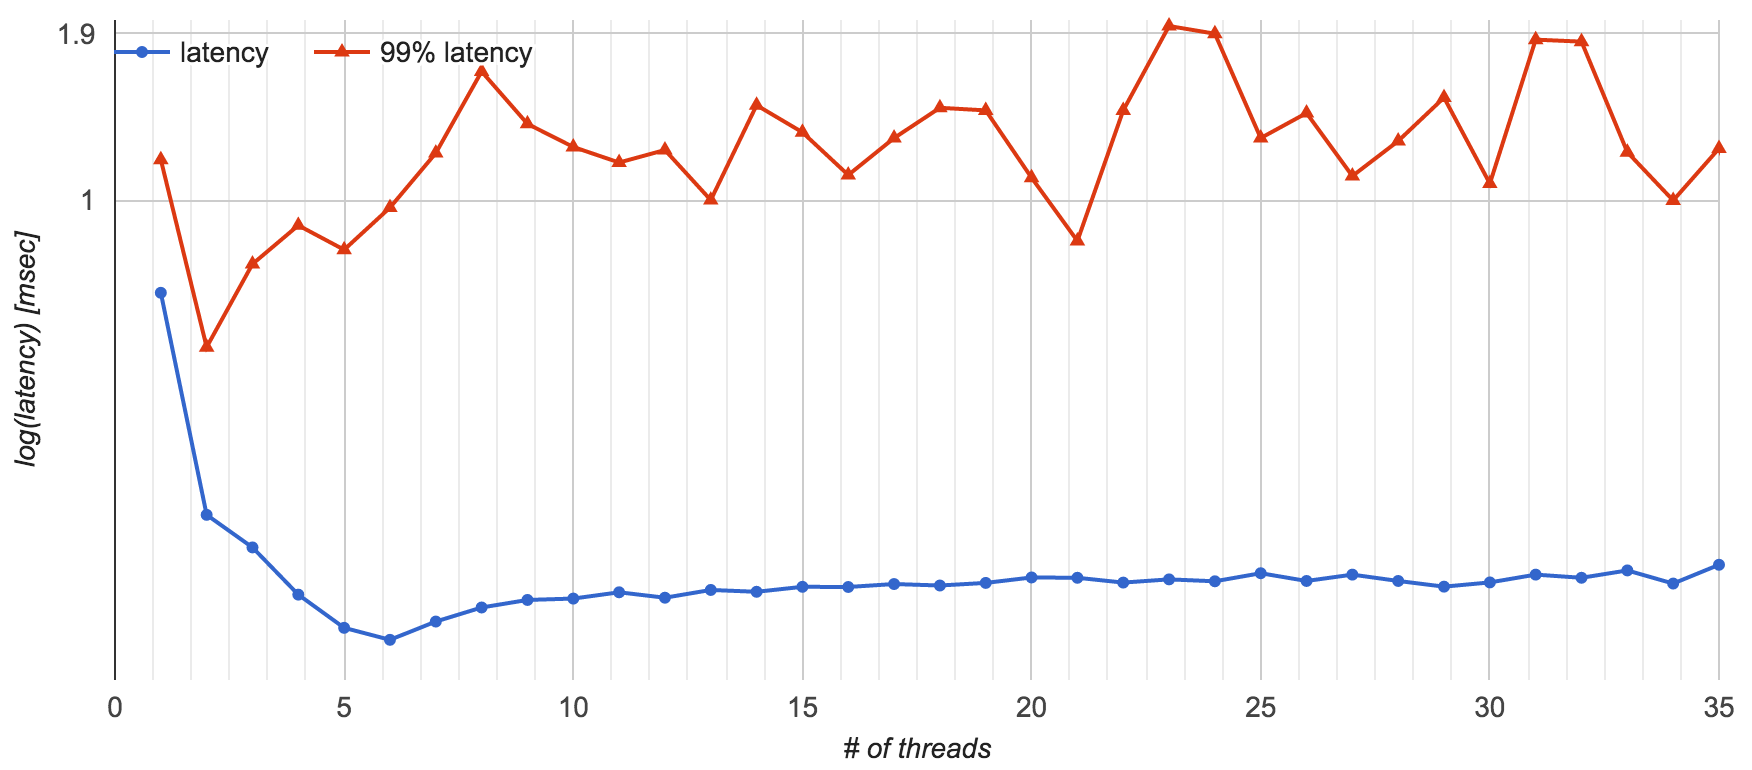
\includegraphics{./res/5_threads_latency.png}
\caption{Memcached Thread Scaling}
\end{figure}

The figure above shows mean and 99th percentile latency against the
number of threads. The lowest mean latency occurs when running 6 threads
of memcached. This corresponds to the expectation of best performance of
using \emph{n} threads with \emph{n} CPU cores. Additionally, less than
6 threads exhibits higher latency than when using 6 cores. A constant
load created against the server and the number of threads less than the
number of CPUs creates a bottleneck where network requests targeted for
a given core are attempted to be processed only by a given core to avoid
an expensive data transfer and a context switch. Consequently, the queue
of requests builds up and overall latency decreases. An increase in the
number of threads allows for a higher throughput due to reduced
bottleneck on request processing. Furthermore, latency increases with
the number of threads as a context switch is required between contexts
in each thread therefore putting additional strain on the operating
system resources.

The 99th percentile lantecy behaves similarly to the mean latency. We
can observe that 99th precentile latency drops below the defined quality
of service when using between 2 and 6 threads. Beyond six threads, 99th
percentile behavior fluctuates above the desired quality of service
boundary.

\begin{figure}[htbp]
\centering
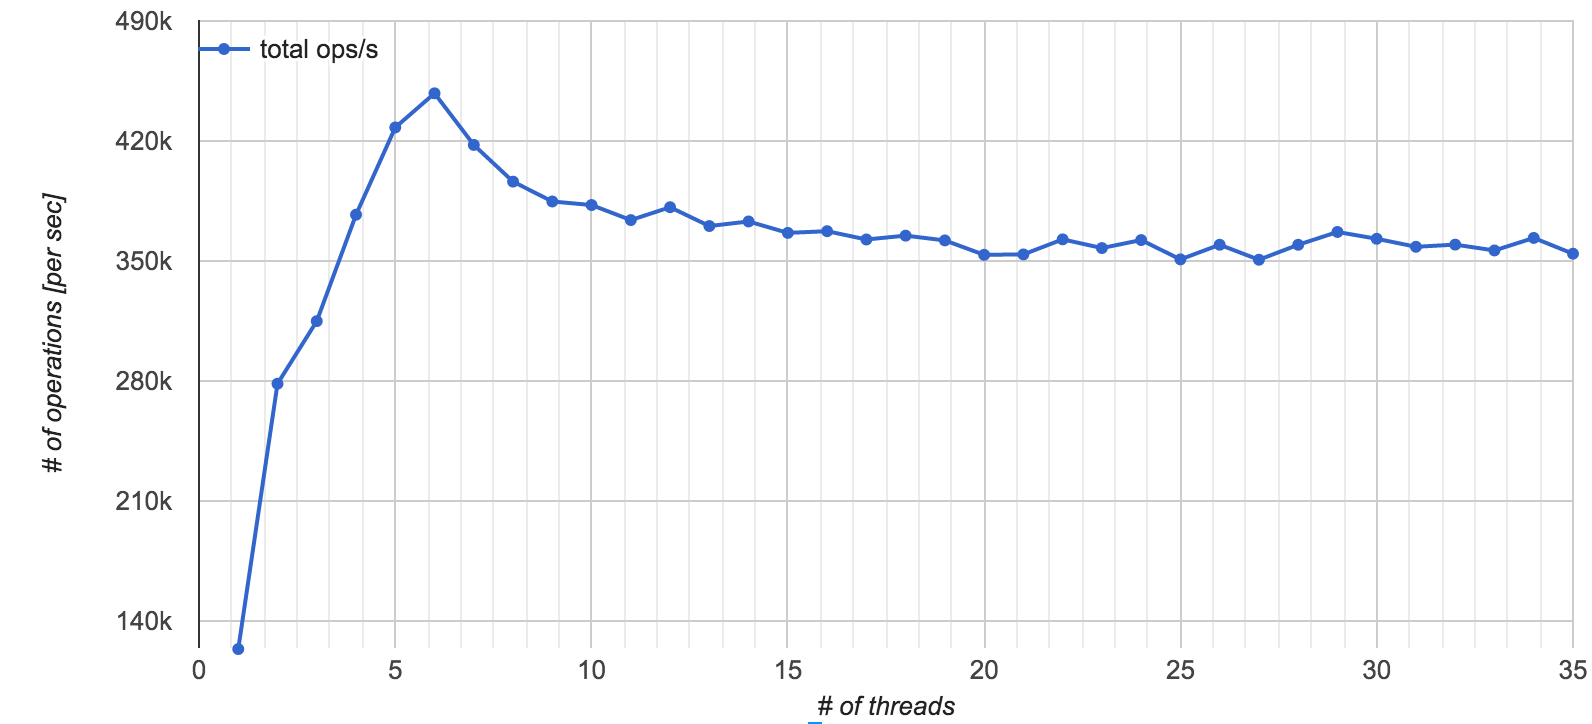
\includegraphics{./res/5_threads_total_ops.png}
\caption{Memcached Thread Total Ops}
\end{figure}

Similarly to latency behavior, throughput is the highest when when
running 6 threads - close to 450k operations per second. This is in
accordance with our expectation as resources are being utilized fully
and overhead from context switching is limited. Additionally, we can see
that throughput incrases drastically between 1 and 6 threads, that is,
from 120k to 450k. A further increase in the number of threads beyond 6
threads only results in a reduction in overall throughput caused by
context switching overheads and operating system resource requirements.

\begin{figure}[htbp]
\centering
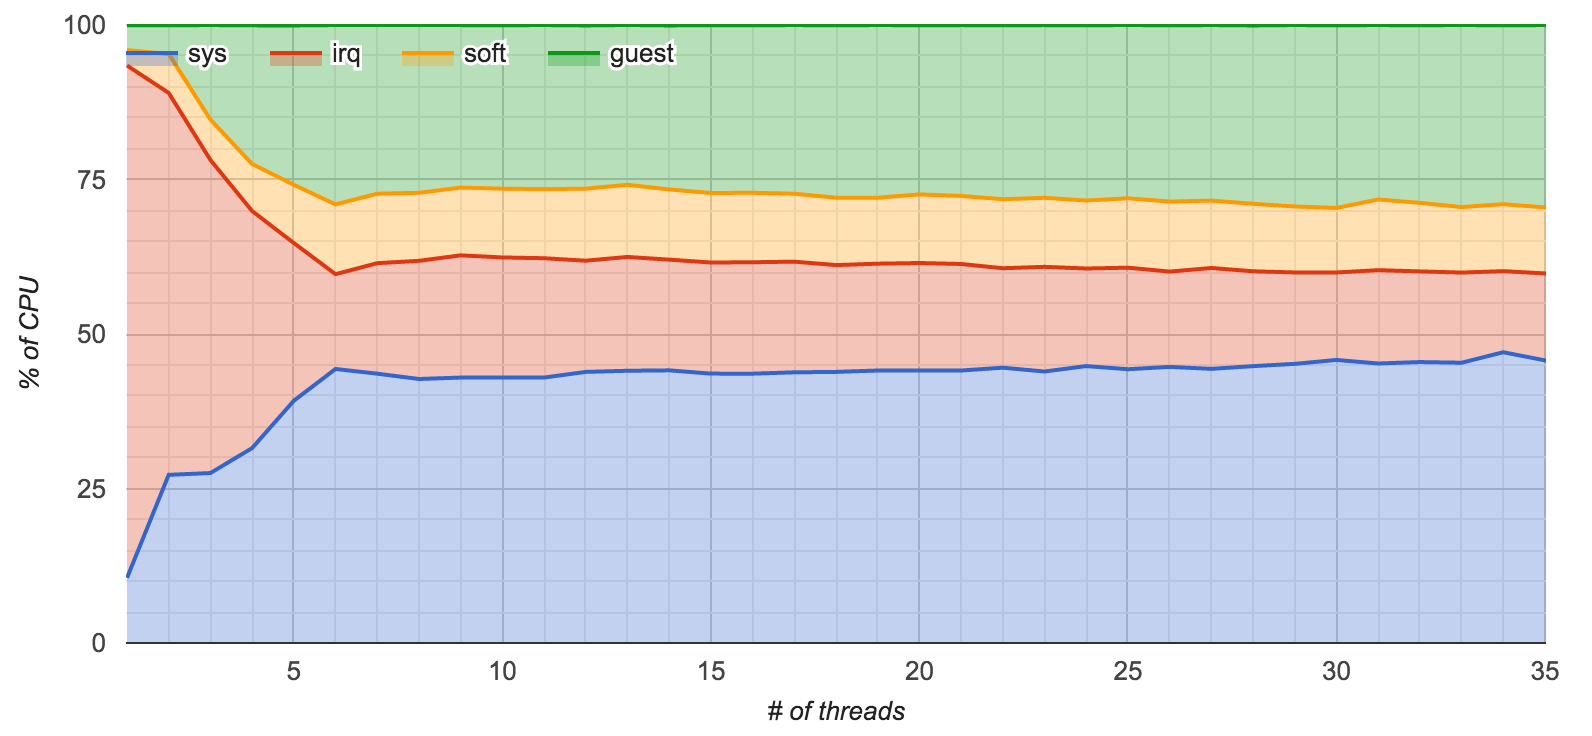
\includegraphics{./res/5_threads_cpu.png}
\caption{Memcached Thread CPU}
\end{figure}

Analysing the CPU usage as we increase the number of threads, we can
observe that initially a large portion of the CPU time is spent
servicing hardware interrupts (\emph{irq}). Therefore, the OS is
handling incoming traffic interrupts from the NIC. As the number of
threads increases, an increasingly larger portion of CPU time is spent
processing system calls and context switching (\emph{sys}). This is
reasonable as a larger number of threads will require context switching
and concurrency management provided by the operating system. We can see
that time spent processing hardware interrupts (\emph{irq}) decreases
which has the effect of increasing latency as packets remained queued up
in the NIC for longer before the OS manages to schedule the interrupt to
be serviced. Furthermore, we can observe that software iterrupts
(\emph{soft}) CPU time progressively increases until we reach 6 threads
and remains stable as the number of threads grows further. The initial
increase is reasonable as we are demanding more threads to processed
simultanesly, past this point the percentage remains stable as we have
reached a saturation point in terms of scalability and server
performance. Finally, memcached (\emph{guest}) follows a similar pattern
as software interrupts. Usage increases until 6 threads are used and
saturates further. This is further indicative of the inability to
efficiently scale the number of threads past the point at which
memcached uses the same number of threads as CPU cores.

\subsection{Thread pinning}\label{thread-pinning}

Thread pinning is the process of assigning a \emph{set\_irq\_affinity}
to each individual thread. As suggested by Leverich and Kozyrakis,
``pinning memcached threads to distinct cores greatly improves load
balance, consequently improving tail latency.'' {[}13{]} and therefore
the reasonable next step in optimizing memcached performance is to
attempt thread pinning and analyse the results obtained.

By default, when a new process is started, its affinity is set to all
available CPUs. We can discover a given process affinity by executing
\texttt{taskset\ -p\ \textless{}pid\textgreater{}} where \texttt{pid} is
the process identifier.

``A Memcache instance started with n threads will spawn n + 1 threads of
which the first n are worker threads and the last is a maintenance
thread used for hash table expansion under high load factor.'' {[}14{]}.
We can discover memcached threads used for request processing using
\texttt{ps\ -p\ \textless{}memcache-process-id\textgreater{}\ -o\ tid=\ -L\ \textbar{}\ sort\ -n\ \textbar{}\ tail\ -n\ +2\ \textbar{}\ head\ -n\ -1}
{[}14{]} and further set their processor affinity using
\texttt{taskset\ -pc\ \textless{}cpu-id\textgreater{}\ \textless{}tid\textgreater{}}
where \emph{} is the thread id discovered previously {[}14{]}.

Given the best performance under QoS constraints of 1ms found in the
previous section is memcached with 6 threads, the following benchmark
will be using this best configuration in order the analyze the impact of
thread pinning.

\begin{figure}[htbp]
\centering
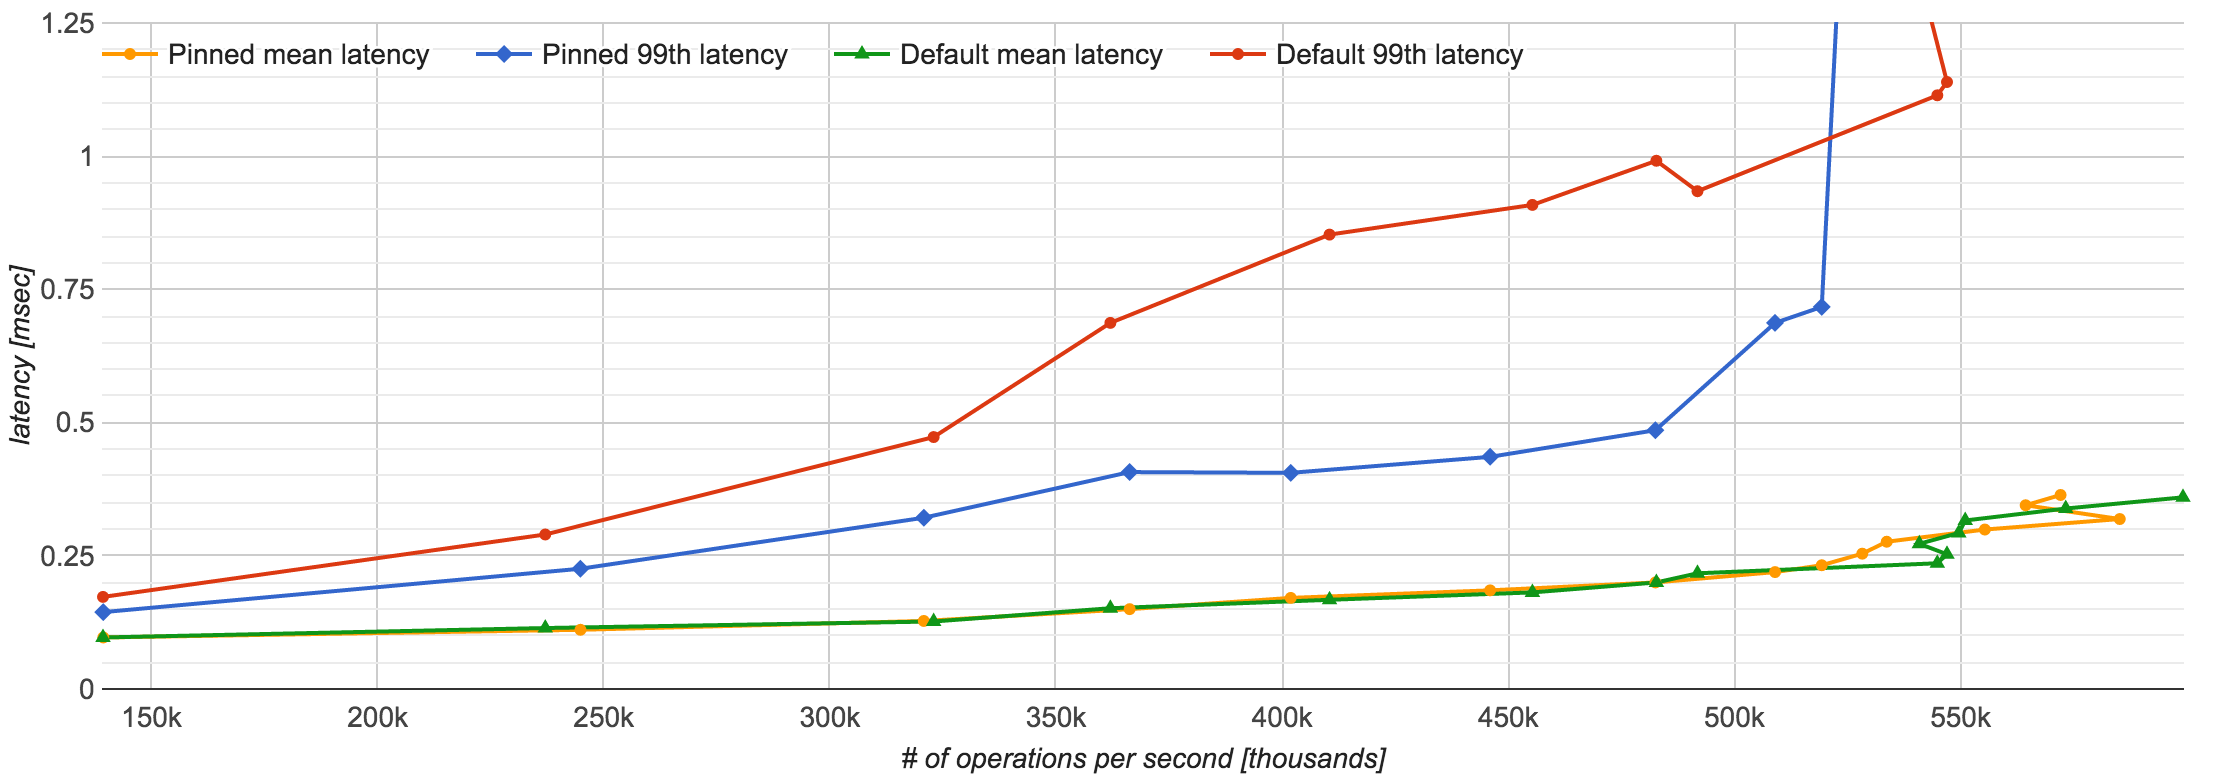
\includegraphics{./res/5_threads_pinned_vs_default.png}
\caption{Memcached Pinned Threads vs Unpinned}
\end{figure}

~

\begin{itemize}
\tightlist
\item
  {[}1{]} {[}memcached.org{]}(http://memcached.org/)
\item
  {[}2{]} An FPGA-based in-line accelerator for Memcached, Maysam
  Lavasani, Hari Angepat, and Derek Chiou
\item
  {[}3{]} {[}New Commands,
  Memcached.org{]}(https://code.google.com/p/memcached/wiki/NewCommands)
\item
  {[}4{]} {[}Scaling memcached at
  Facebook{]}(https://www.facebook.com/notes/facebook-engineering/scaling-memcached-at-facebook/39391378919/)
\item
  {[}5{]}
\item
  {[}6{]} {[}Amazon ElastiCache{]}(http://aws.amazon.com/elasticache/)
\item
  {[}7{]} Workload Analysis of a Large-Scale Key-Value Store, Berk
  Atikoglu, Yuehai Xu, Eitan Frachtenberg, Song Jiang, Mike Paleczny
\item
  {[}8{]} http://investor.fb.com/releasedetail.cfm?ReleaseID=908022
\item
  {[}9{]} {[}Twemproxy{]}(https://github.com/twitter/twemproxy)
\item
  {[}10{]} {[}Enhancing the Scalability of
  Memcached{]}(https://software.intel.com/sites/default/files/m/0/b/6/1/d/45675-memcached\_05172012.pdf)
\item
  {[}11{]} Thin Servers with Smart Pipes: Designing SoC Accelerators for
  Memcached - Kevin Lim, David Meisner, Ali G. Saidi, Parthasarathy
  Ranganathan, Thomas F. Wenisch
\item
  {[}12{]} MICA: A Holistic Approach to Fast In-Memory Key-Value Storage
\item
  {[}13{]} Reconciling High Server Utilization and Sub-millisecond
  Quality-of-Service, Jacob Leverich Christos Kozyrakis
\item
  {[}14{]} Filling The Pipe: A Guide To Optimising Memcache Performance
  On Solarflare Hardware
\end{itemize}
